\section{Darba punkta nodrošināšanas sistēmas izstrāde}
Šajā nodaļā tiek aprakstīta izstrādes plates modifikācija un testēšana, izstrādātie līdzstrāvas sprieguma pārveidotāji, industriālā barošanas avota vadības, strāvas mērīšanas, ieslēgšanas/izslēgšanas elektriskā principiālā shēmas. Daļas, kas nodrošina darba punkta iestatīšanas/atiestatīšanas funkciju.
\subsection{Monitoringa izstrādes plates modifikācija un integrēšana}
Lai ātrāk iegūtu vēlamo rezultātu, tika iegādāta izstrādes plate ar izvēlēto monitorēšanas integrālo shēmu EVAL-AD7293 \cite{eval_board} ar AD piedāvātu vadības sistēmu EVAL-SDP-CB1Z \cite{eval_board_mcu}.
\begin{figure}[H]
	\centering
    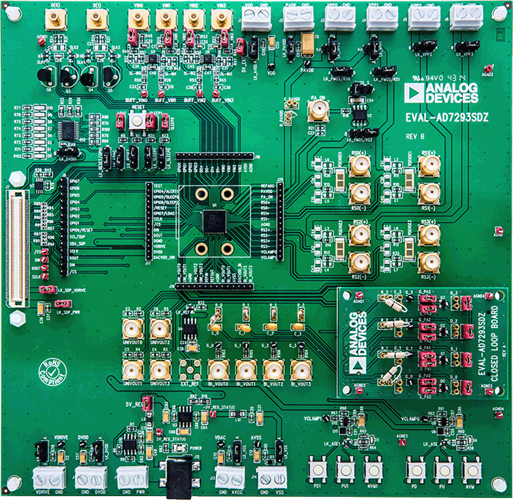
\includegraphics[width=0.5\textwidth]{pictures/EVAL-AD7293SDZ_TOP-web.png}\hspace{1cm}
    \caption{AD7293 izstrādes plate}
\end{figure}
\begin{figure}[H]
	\centering
    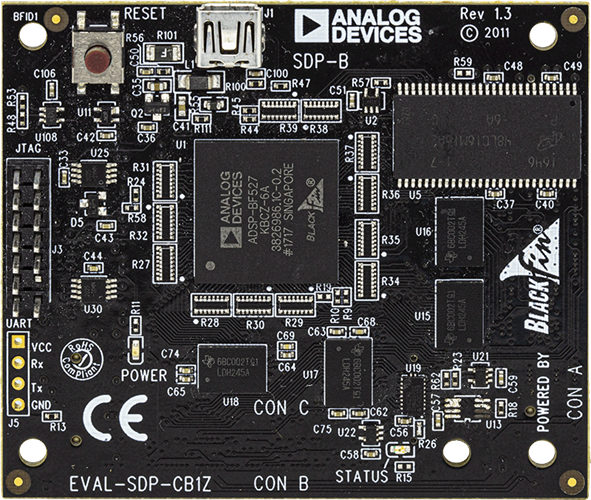
\includegraphics[width=0.5\textwidth]{pictures/EVAL-SDP-B-top-web.png}\hspace{1cm}
    \caption{Vadības sistēma monitorēšanas izstrādes platei}
\end{figure}
Šīs sistēmas pārbaudei tika izmantota AD lietojumprogramma, kas sniedz vispārīgu pārskatu par sistēmas funkcionalitāti.
\begin{figure}[H]
	\centering
    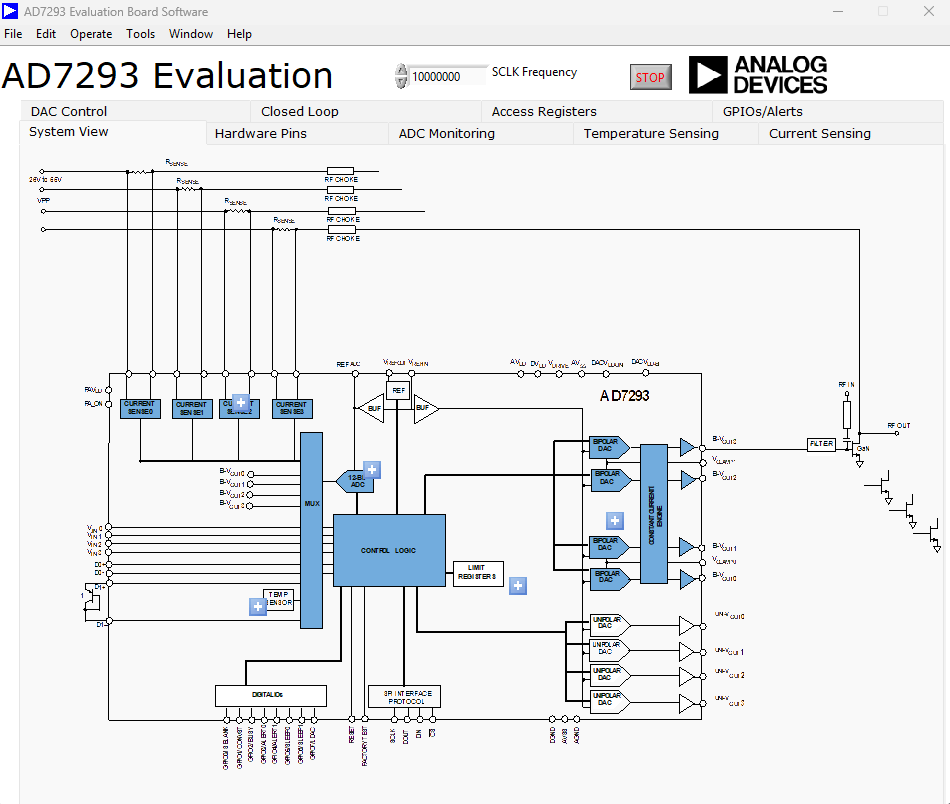
\includegraphics[width=0.6\textwidth]{pictures/eval-soft.png}\hspace{1cm}
    \caption{AD7293 testēšanas lietojumprogramma}
\end{figure}
Sekojot datu lapā pieejamai informācijai tika nodrošināta reģistru konfigurācijas secība un sasniegta vēlamā funkcionalitāte darba punkta iestatīšanai un atiestatīšanai.\\
Pēc nepieciešamās funkcionalitātes nodrošināšanas tika veiktas izstrādes plates modifikācijas - atlodēti SMA konektori, lai varētu pielodēt strāvas monitorēšanas sistēmas izvadus un ieslēgšanas/izslēgšanas sistēmas vadības izvadu, samainīti savienotājelementi, pievienoti barošanas avoti un pievienots digitālās loģikas analizators, lai monitorētu SPI saskarni.
\begin{figure}[H]
	\centering
    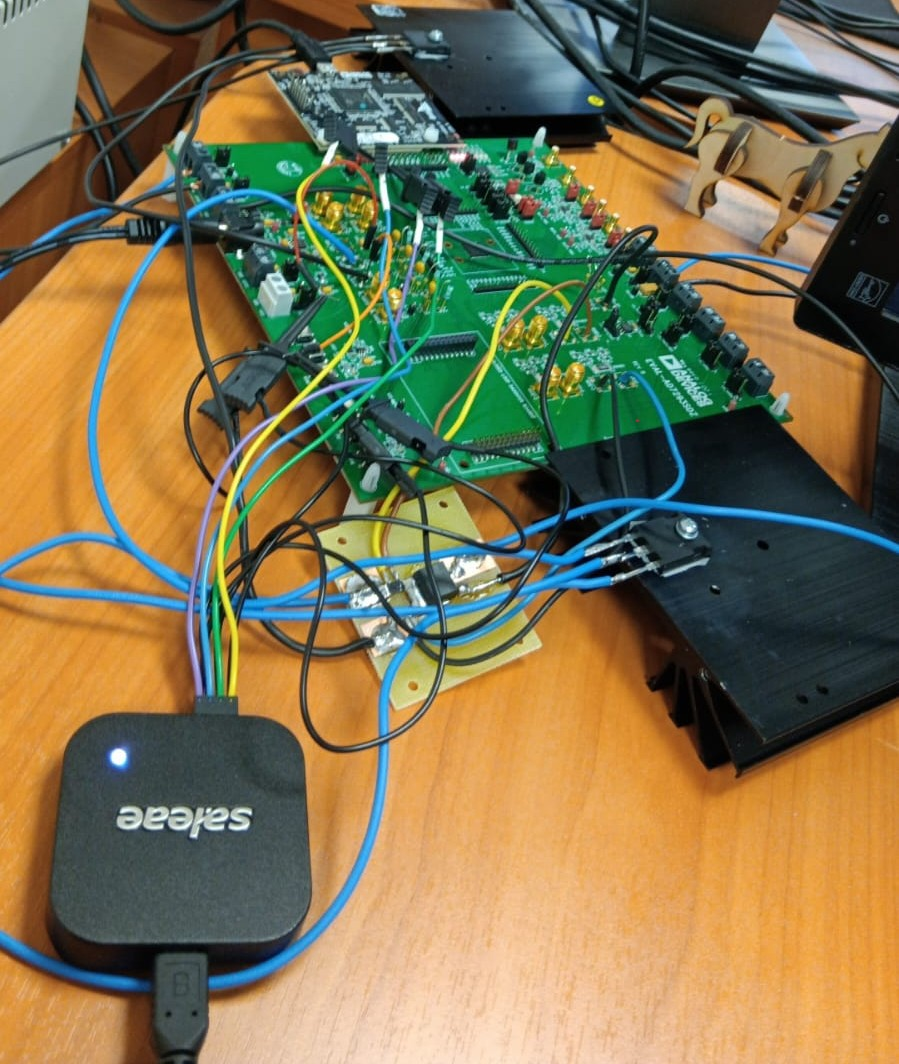
\includegraphics[width=0.5\textwidth]{pictures/daf.jpg}\hspace{1cm}
    \caption{Testa stends ar testa lauktranzistoriem}
\end{figure}
Tad tika sasniegts vēlamais rezultāts ar darba punkta iestatīšanu un atiestatīšanu.
\subsection{Sprieguma pārveidotāji, temperatūras sensora un 24 V barošanas avota vadības shēmas}
Tika izvēlēti lineārie sprieguma stabilizatori 5 un 9 V līnijām, neskatoties uz zemo efektivitāti, salīdzinot ar impulsa tipa sprieguma stabilizatoriem, tie nerada trokšņus izejā. Lineārie sprieguma stabilizatori tiek slēgti virknē, lai palielinātu 5 V regulātora efektivitāti, samazinot sprieguma kritumu uz tā. 12 V tiek pārveidots uz 9 V un no 9 V tiek pārveidots uz 5 V.  
\begin{figure}[H]
	\centering
    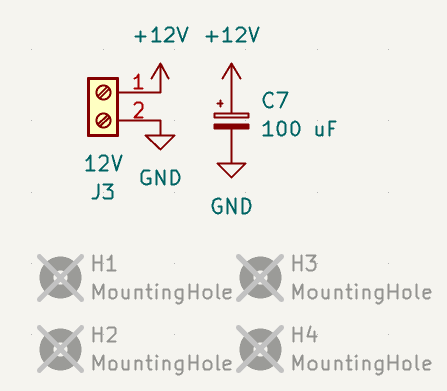
\includegraphics[width=0.6\textwidth]{pictures/inputs.png}\hspace{1cm}
    \caption{Ievadi, elektrolītiskais kondesators un urbjcaurumi}
\end{figure}
J3 terminālbloks ir paredzēts, lai varētu pieslēgt industriālo 12 V barošanas avotu. C7 elektrolītiskais kondensators paredzēts, lai mazinātu ieejas pulsācijas. H1, H2, H3 un H4 urbjcaurumi paredzēti, lai iespiedplati varētu iestiprināt korpusā.
\begin{figure}[H]
	\centering
    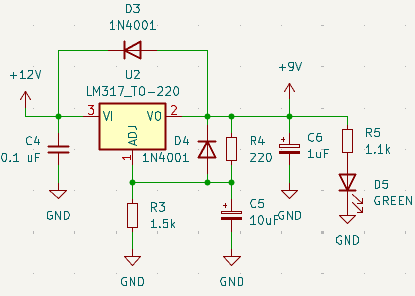
\includegraphics[width=0.6\textwidth]{pictures/9v.png}\hspace{1cm}
    \caption{12 V uz 9 V pārveidotais}
\end{figure}
\begin{figure}[H]
	\centering
    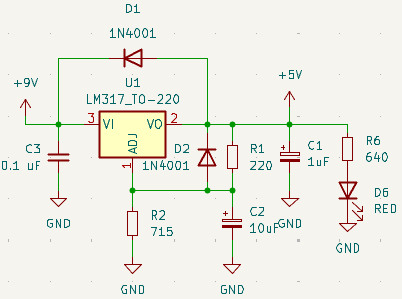
\includegraphics[width=0.6\textwidth]{pictures/5v.png}\hspace{1cm}
    \caption{9 V uz 5 V pārveidotais}
\end{figure}
Sprieguma iestatīšanai tiek izmantota atgriezeniskā saite, ko veido rezistori R1, R2, R3 un R4. Ķēdē tiek izmantoti keramiskie kondensatori C1, C3, C4 un C6. keramiskie un elektrolītiskie kondensatori ir vajadzīgi, lai mazinātu barošanas pulsācijas. R6 un R5 ir strāvas ierobežojošie rezistori D5 un D6 gaismas diodēm. D1, D2, D3 un D4 taisngriežu diodes paredzētas, lai neļautu C2 un C5 kondensatoriem izlādēties lineārā sprieguma izejā.
\begin{figure}[H]
	\centering
    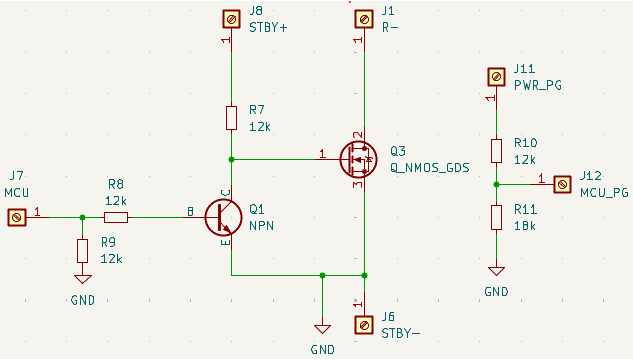
\includegraphics[width=0.6\textwidth]{pictures/24_control_detection.png}\hspace{1cm}
    \caption{24 V barošanas avota vadības sistēmu}
\end{figure}
J7 izvads paredzēts, lai varētu pieslēgt mikrokontrolliera vadības signālu. R8 ir paredzēts strāvas ierobežošanai NPN bipolārajam tranzistoram. R9 ir zema līmeņa piesaistes rezistors, lai pārejas procesā netiktu atvērts tranzistors. R7 rezistors ir paredzēts strāvas ierobežošanai un augsta signāla līmeņa piesaistei pie N kanāla lauktranzistora aizvara. J8, J1 un J6 izvadi paredzēti, lai varētu vadīt 24 V industriālo barošanas avotu. J11 ir paredzēts barošanas avota stāvokļa pieslēgvieta, kur R10 un R11 rezistori ir sprieguma dalītāji, lai varētu veikt sprieguma nolasi ar mikrokontrolliera.
\begin{figure}[H]
	\centering
    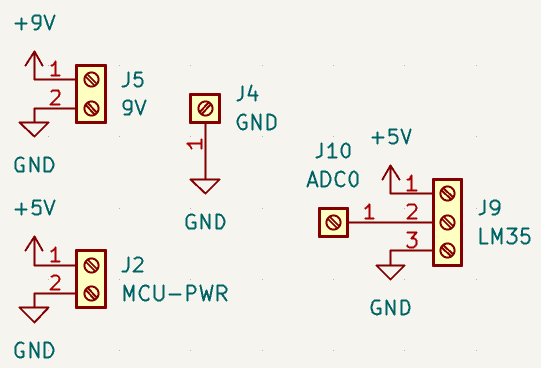
\includegraphics[width=0.6\textwidth]{pictures/outputs.png}\hspace{1cm}
    \caption{Pieslēgvietas MCU, temperatūras un patērētājiem}
\end{figure}
J5 un J2 terminālbloks paredzēts, lai varētu nodrošināt 9 V un 5 V barošanu patērētājiem. J9 terminālbloks paredzēts temperatūras sensora pieslēgšanai. J10 ir izvads, paredzēts mikrokontroliera ADC pieslēgvietai.
\begin{figure}[H]
	\centering
    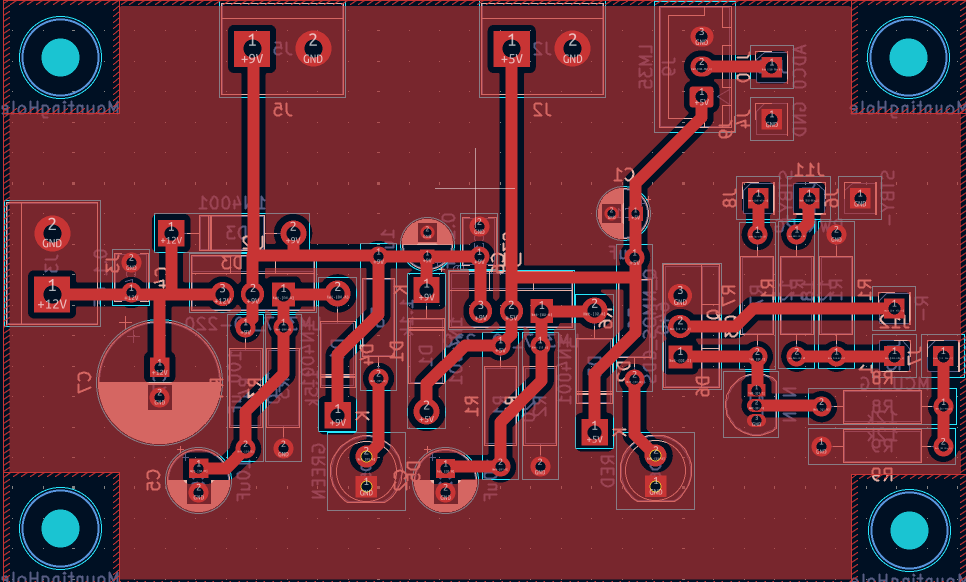
\includegraphics[width=0.6\textwidth]{pictures/power_board.png}\hspace{1cm}
    \caption{Iespiedplate lietojumprogrammatūrā "KiCad"}
\end{figure}
 Iespiedplate tika trasēta vienā slānī. Komponentes tika izvietotas pēc iespējas blīvāk, lai samazinātu iespiedplates izmērus. Tika izmantotas THT komponentes. Iespiedplate tika izfrēzēta ar augstskolā pieejamo frēzi.
\subsection{Strāvas mērīšanas iespiedplate ar ieslēgšanas/izslēgšanas slēdzi}
\begin{figure}[H]
	\centering
    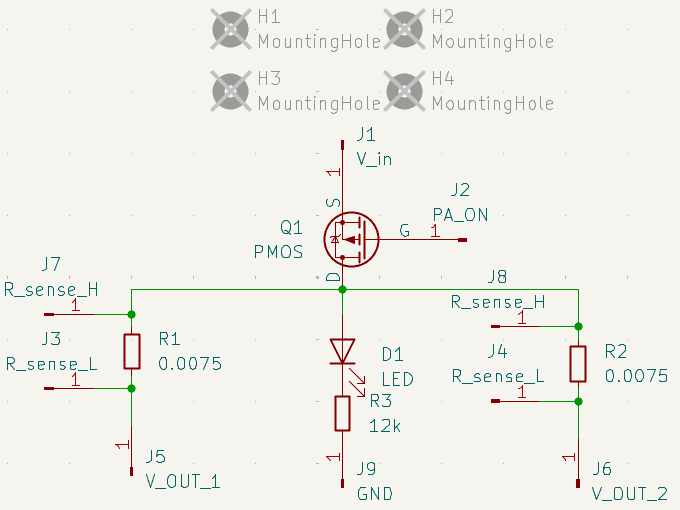
\includegraphics[width=0.6\textwidth]{pictures/shunt_resistors.png}\hspace{1cm}
    \caption{Strāvas mērīšanas shematiskais zīmējums}
\end{figure}
J1 terminālbloks ir 24 V pieslēgvietas nodrošināšanai. Q1 P kanāla lauktranzistors tiek izmantots slēdža režīmā, kas tiek kontrolēts ar AD7293 monitorēšanas integrālo shēmu, kas tiek pievadīts caur J2 termināli. R1 un R2 ir šunta rezistori strāvas mērīšanai. Šunta rezistori tika aprēķināti pēc izvēlētā mērīšanas diapazona AD7293 un maksimālās strāvas R <= 0.025/3 . J3, J4, J7 un J8 izvadi ir paredzēti, lai pieslēgtu strāvas mērīšanas sistēmu. D1 gaismas diodē ir paredzēta sistēmas stāvokļa identificēšanai. R3 rezistors ir paredzēts strāvas ierobežošanai, lai pasargātu gaismas diodi. J9 izvads paredzēts zemējuma nodrošināšanai.
\begin{figure}[H]
	\centering
    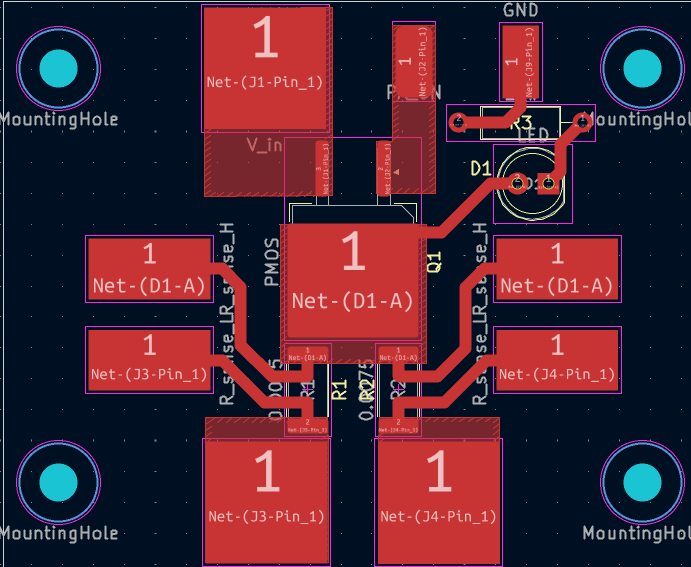
\includegraphics[width=0.6\textwidth]{pictures/shunt_resistors_board.png}\hspace{1cm}
    \caption{Iespiedplate lietojumprogrammatūrā "KiCad"}
\end{figure}
Tika izstrādāta vienslāņu plate ar blīvu komponenšu izvietojumu un attiecīgu jaudas celiņu platumiem. Tā tika izfrēzēta ar VeA pieejamo frēzi.
